% Provenance (never printed): cycle 4 SVT, "La planete Terre, l'environnement
% et l'action humaine": the relief as a balance between uplift and erosion;
% landforms of the wind, the sea and dissolution; reading a landscape; see
% sources/book1/PROVENANCE.md. Book 1, grade 9, chapter 4.
% Vocabulary guard: owns uplift, dune, cliff, beach and spit (with longshore
% drift), karst (with cave and sinkhole). Landscape and landform are g1's;
% weathering, erosion, deposition, meander and delta are g5's; relief is
% g4's; plates and mountain building are g7's; U-shaped valley and moraine
% are g8's; limestone and the acid test are g6's; acids are the chemistry
% books' (recalled in prose). Contour lines are g9.5's (not used here).
% "Normal fault" and the destruction of mountains are Book 2's.
\chapter{As formas de relevo}\label{ch:g9:landforms}

Na costa sul da Inglaterra, as \omterm{def:g9:landforms:cliff}{falésias} brancas das Seven Sisters caem
direto no \omterm{def:g2:water-on-earth:ocean}{mar}. Num ano normal, elas perdem até um metro. No inverno de
2014, as \omterm{def:g5:natural-hazards:storm}{tempestades} tiraram das \omterm{def:g9:landforms:cliff}{falésias} de Birling Gap, em dois meses,
tanto quanto elas costumam perder em sete anos. O giz dessas \omterm{def:g9:landforms:cliff}{falésias} foi
um dia \omterm{def:g3:stones-pebbles-sand:sand}{lama} no fundo de um \omterm{def:g2:water-on-earth:ocean}{mar}, feita das minúsculas placas de algas
microscópicas que viviam na sua água. Hoje ele se ergue como uma muralha
de \omterm{def:g3:stones-pebbles-sand:rock}{rocha} branca que as ondas fazem recuar um pouco mais a cada ano. Por
que a terra tem as formas que tem, e por que algumas delas mudam tão
depressa?
% ledger: nt:birling-2014, sdnp:birling, nasa:coccoliths

\begin{omfigure}
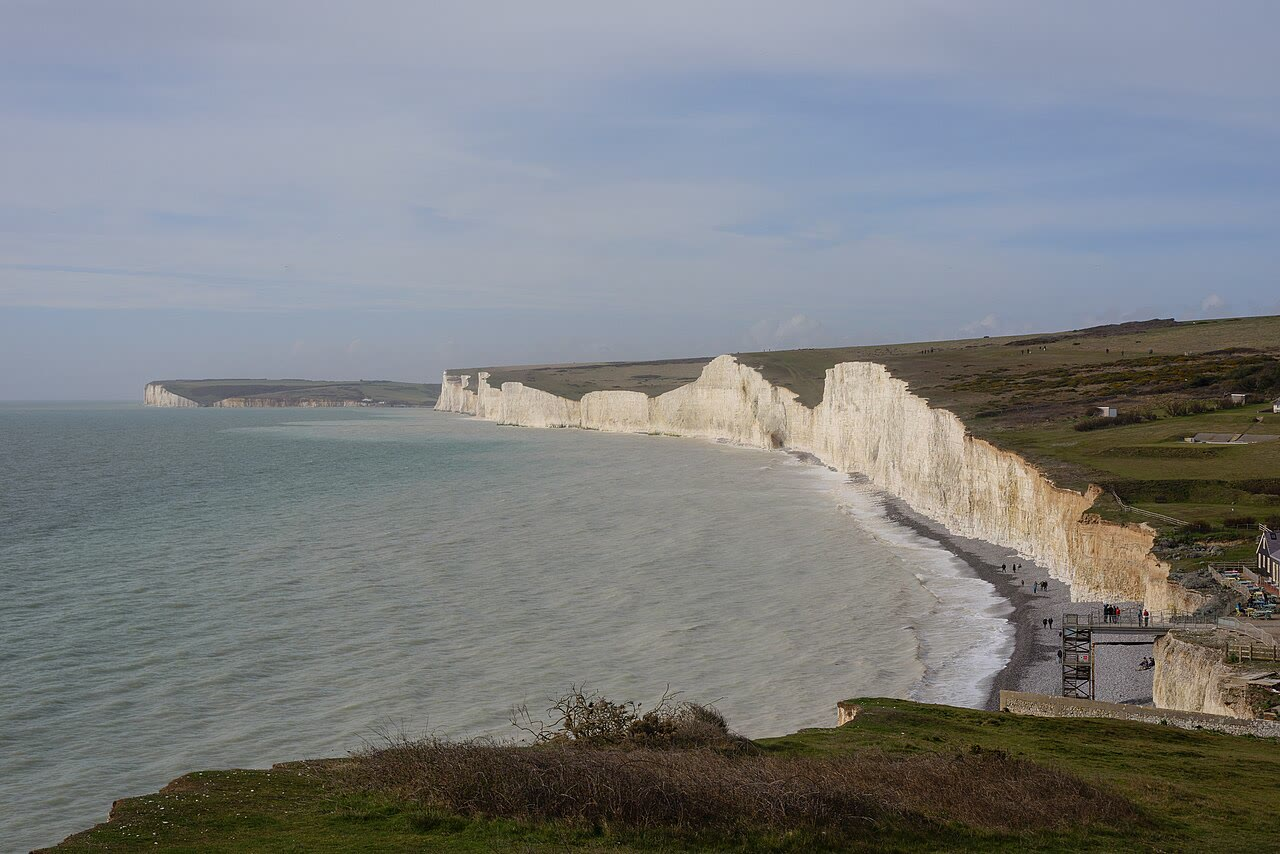
\includegraphics[width=\linewidth]{images/book1/g9-seven-sisters.jpg}

{\small As Seven Sisters, \omterm{def:g9:landforms:cliff}{falésias} de giz na costa de East Sussex
(Inglaterra), com as casas de Birling Gap em primeiro plano. As \omterm{def:g9:landforms:cliff}{falésias}
recuam sob a ação do \omterm{def:g2:water-on-earth:ocean}{mar}, e desmoronamentos de \omterm{def:g3:stones-pebbles-sand:rock}{rocha} acontecem a qualquer
momento. Ao pé delas, há uma \omterm{def:g9:landforms:beach}{praia} de \omterm{def:g3:stones-pebbles-sand:pebble}{seixos}. Fotografia de Arild Vågen,
2017 (CC BY-SA 4.0, via Wikimedia Commons).}
% ledger: commons:seven-sisters, sdnp:birling
\label{fig:g9:landforms:seven-sisters}
\end{omfigure}

\begin{recall}
Uma \emph{\omterm{def:g1:landscapes-around-us:landform}{forma de relevo}} é uma forma da superfície da terra: um morro,
um \omterm{def:g1:landscapes-around-us:landform}{vale}, uma \omterm{def:g1:landscapes-around-us:landform}{planície}, uma \omterm{def:g9:landforms:cliff}{falésia} (\cref{ch:g1:landscapes-around-us}). O
\omterm{def:g4:world-physical-map:relief}{relevo} é a forma do terreno em altura (\cref{ch:g4:world-physical-map}).
O \omterm{def:g5:water-shapes-the-land:weathering}{intemperismo} fragmenta a \omterm{def:g3:stones-pebbles-sand:rock}{rocha}, a \omterm{def:g5:water-shapes-the-land:erosion}{erosão} a desgasta e a leva embora, e a
\omterm{def:g5:water-shapes-the-land:deposition}{deposição} a assenta em outro lugar (\cref{ch:g5:water-shapes-the-land}).
As \omterm{def:g7:plate-tectonics:plate}{placas} erguem \omterm{def:g4:world-physical-map:range}{cordilheiras} onde colidem (\cref{ch:g7:plate-tectonics});
as \omterm{def:g8:ice-on-earth:glacier}{geleiras} escavam \omterm{def:g8:ice-on-earth:glacial-landforms}{vales em U} (\cref{ch:g8:ice-on-earth}); o calcário
efervesce sob uma gota de ácido diluído (\cref{ch:g6:rocks-and-minerals}).
Em química, você aprende que os ácidos atacam o calcário e liberam gás
carbônico.
\end{recall}

\section{O relevo: um equilíbrio entre soerguimento e erosão}

Dois tipos de forças modelam o \omterm{def:g4:world-physical-map:relief}{relevo}. De dentro, os movimentos das \omterm{def:g7:plate-tectonics:plate}{placas}
elevam o terreno. De fora, a água, o gelo, o vento e o \omterm{def:g2:water-on-earth:ocean}{mar} o desgastam.

\begin{definition}[Soerguimento]\label{def:g9:landforms:uplift}
O \emph{soerguimento}\index{soerguimento} é a subida lenta das \omterm{def:g3:stones-pebbles-sand:rock}{rochas} e da
superfície do terreno de uma região, provocada por forças do interior da
Terra, como a colisão de duas \omterm{def:g7:plate-tectonics:plate}{placas}.
\end{definition}

O \omterm{def:g9:landforms:uplift}{soerguimento} é lento na escala de uma vida, mas rápido na escala da
Terra. A Índia colidiu com a Ásia há cerca de 50~milhões de anos, e o
planalto do Tibete, atrás do Himalaia, ganhou a maior parte da sua
\omterm{def:g4:world-physical-map:altitude}{altitude}, cerca de \qty{4600}{m}, nos últimos 10~milhões de anos. Em
média, isso dá
$4600 \div 10^7 = 4.6 \times 10^{-4}$~m, ou cerca de \qty{0.5}{mm} por
ano: menos que a espessura de uma unha, mas mantido por milhões de anos.
% ledger: usgs:himalaya (rate computed in figdata/grade-9/cliff_retreat.py, tibet_rate_mm_yr)

Assim que o terreno sobe, a \omterm{def:g5:water-shapes-the-land:erosion}{erosão} o ataca. Quanto mais alto e mais
íngreme o terreno, mais depressa os \omterm{def:g1:landscapes-around-us:water}{rios}, as \omterm{def:g8:ice-on-earth:glacier}{geleiras} e os desmoronamentos
levam a \omterm{def:g3:stones-pebbles-sand:rock}{rocha} embora. A altura de uma \omterm{def:g4:world-physical-map:range}{cordilheira} num dado momento é o
resultado de uma disputa: o que o \omterm{def:g9:landforms:uplift}{soerguimento} traz para cima, menos o
que a \omterm{def:g5:water-shapes-the-land:erosion}{erosão} leva embora.

\begin{omfigure}
\begin{tikzpicture}[font=\footnotesize, >={Stealth[length=2mm]}]
  % panel 1: uplift faster than erosion
  \begin{scope}
    \fill[black!13] (0,0) -- (0.5,0) .. controls (1.1,1.0) and (1.5,2.0) .. (1.8,2.2)
      .. controls (2.1,2.0) and (2.5,1.0) .. (3.1,0) -- (3.6,0) -- (3.6,-0.5) -- (0,-0.5) -- cycle;
    \draw[black!60] (0,0) -- (0.5,0) .. controls (1.1,1.0) and (1.5,2.0) .. (1.8,2.2)
      .. controls (2.1,2.0) and (2.5,1.0) .. (3.1,0) -- (3.6,0);
    \draw[black!60, dashed] (0.7,0) .. controls (1.2,0.8) and (1.5,1.5) .. (1.8,1.6)
      .. controls (2.1,1.5) and (2.4,0.8) .. (2.9,0);
    \foreach \x in {1.2,1.8,2.4} \draw[->, omWarm, line width=1.4pt] (\x,-0.45) -- ++(0,1.0);
    \draw[->, omRiver, thick] (2.15,1.6) -- ++(0.35,-0.3);
    \node[align=center, anchor=north] at (1.8,-0.6) {soerguimento mais rápido\\que a erosão: o relevo sobe};
  \end{scope}
  % panel 2: uplift equals erosion
  \begin{scope}[xshift=4.4cm]
    \fill[black!13] (0,0) -- (0.5,0) .. controls (1.1,1.0) and (1.5,1.8) .. (1.8,1.9)
      .. controls (2.1,1.8) and (2.5,1.0) .. (3.1,0) -- (3.6,0) -- (3.6,-0.5) -- (0,-0.5) -- cycle;
    \draw[black!60] (0,0) -- (0.5,0) .. controls (1.1,1.0) and (1.5,1.8) .. (1.8,1.9)
      .. controls (2.1,1.8) and (2.5,1.0) .. (3.1,0) -- (3.6,0);
    \foreach \x in {1.2,1.8,2.4} \draw[->, omWarm, line width=1.4pt] (\x,-0.45) -- ++(0,0.6);
    \draw[->, omRiver, thick] (2.05,1.6) -- ++(0.55,-0.5);
    \draw[->, omRiver, thick] (1.55,1.6) -- ++(-0.55,-0.5);
    \node[align=center, anchor=north] at (1.8,-0.6) {soerguimento igual à erosão:\\a altura não muda};
  \end{scope}
  % panel 3: no more uplift
  \begin{scope}[xshift=8.8cm]
    \fill[black!13] (0,0) -- (0.4,0) .. controls (1.1,0.5) and (1.5,0.95) .. (1.8,1.0)
      .. controls (2.1,0.95) and (2.5,0.5) .. (3.2,0) -- (3.6,0) -- (3.6,-0.5) -- (0,-0.5) -- cycle;
    \draw[black!60] (0,0) -- (0.4,0) .. controls (1.1,0.5) and (1.5,0.95) .. (1.8,1.0)
      .. controls (2.1,0.95) and (2.5,0.5) .. (3.2,0) -- (3.6,0);
    \draw[black!60, dashed] (0.5,0) .. controls (1.1,1.0) and (1.5,1.8) .. (1.8,1.9)
      .. controls (2.1,1.8) and (2.5,1.0) .. (3.1,0);
    \draw[->, omRiver, thick] (2.05,0.95) -- ++(0.55,-0.5);
    \draw[->, omRiver, thick] (1.55,0.95) -- ++(-0.55,-0.5);
    \node[align=center, anchor=north] at (1.8,-0.6) {sem soerguimento: a erosão\\rebaixa o relevo};
  \end{scope}
  % key
  \draw[->, omWarm, line width=1.4pt] (13.2,1.2) -- ++(0,0.6) node[right, black] {soerguimento};
  \draw[->, omRiver, thick] (13.2,0.7) -- ++(0.35,-0.3) node[right, black] {erosão};
  \draw[black!60, dashed] (13.1,-0.1) -- ++(0.5,0) node[right, black] {perfil anterior};
\end{tikzpicture}

{\small O \omterm{def:g4:world-physical-map:relief}{relevo} como um equilíbrio (um esboço, fora de escala). O
\omterm{def:g9:landforms:uplift}{soerguimento} eleva as \omterm{def:g3:stones-pebbles-sand:rock}{rochas}; a \omterm{def:g5:water-shapes-the-land:erosion}{erosão} as leva para os \omterm{def:g1:landscapes-around-us:landform}{vales} e para o
\omterm{def:g2:water-on-earth:ocean}{mar}. Uma \omterm{def:g4:world-physical-map:range}{cordilheira} continua crescendo enquanto o \omterm{def:g9:landforms:uplift}{soerguimento} vence;
quando as \omterm{def:g7:plate-tectonics:plate}{placas} param de empurrar, a \omterm{def:g5:water-shapes-the-land:erosion}{erosão} a desgasta lentamente até
virar morros.}
\label{fig:g9:landforms:balance}
\end{omfigure}

Os \omterm{def:g1:landscapes-around-us:water}{rios} (\cref{ch:g5:water-shapes-the-land}) e as \omterm{def:g8:ice-on-earth:glacier}{geleiras}
(\cref{ch:g8:ice-on-earth}) são os grandes escultores das \omterm{def:g1:landscapes-around-us:landform}{montanhas}. O
resto deste capítulo acompanha três outros agentes, que fazem \omterm{def:g1:landscapes-around-us:landform}{formas de
relevo} próprias: o vento, o \omterm{def:g2:water-on-earth:ocean}{mar} e a água que dissolve a \omterm{def:g3:stones-pebbles-sand:rock}{rocha}.

\section{As formas feitas pelo vento: as dunas}

Onde há poucas plantas, muita \omterm{def:g3:stones-pebbles-sand:sand}{areia} solta e vento forte, o vento pode
levantar a \omterm{def:g3:stones-pebbles-sand:sand}{areia} e amontoá-la em morros: nos \omterm{def:g5:weather-and-climate:desert}{desertos} e atrás das \omterm{def:g9:landforms:beach}{praias}
arenosas.
% ledger: nps:aeolian

\begin{definition}[Duna]\label{def:g9:landforms:dune}
Uma \emph{duna}\index{duna} é um monte ou uma crista de \omterm{def:g3:stones-pebbles-sand:sand}{areia} solta
amontoada pelo vento. A sua encosta voltada para o vento é longa e suave;
o seu lado oposto, a \emph{face de avalanche}\index{face de avalanche},
é curto e íngreme.
\end{definition}
% ledger: nps:aeolian, nmt:barchan

Uma \omterm{def:g9:landforms:dune}{duna} se move. O vento faz os grãos rolarem e saltarem encosta suave
acima; na crista, eles se acumulam até que o monte fique íngreme demais, e
uma pequena avalanche de \omterm{def:g3:stones-pebbles-sand:sand}{areia} escorrega pela \omterm{def:g9:landforms:dune}{face de avalanche}. Grão após
grão, a \omterm{def:g3:stones-pebbles-sand:sand}{areia} é tirada do lado do vento e depositada do lado oposto, e a
\omterm{def:g9:landforms:dune}{duna} inteira avança no sentido do vento sem nunca ser levantada. As \omterm{def:g9:landforms:dune}{dunas}
raramente ficam sozinhas: elas cobrem campos inteiros.
% ledger: nmt:barchan, nps:aeolian

Onde o vento sopra sempre da mesma direção e a \omterm{def:g3:stones-pebbles-sand:sand}{areia} não é abundante
demais, as \omterm{def:g9:landforms:dune}{dunas} tomam a forma de um crescente, uma \emph{barcana}: o seu
nariz arredondado fica de frente para o vento e os seus dois chifres
apontam no sentido do vento. Os chifres contêm menos \omterm{def:g3:stones-pebbles-sand:sand}{areia} que o meio,
então se movem mais depressa e se estendem à frente da \omterm{def:g9:landforms:dune}{duna}.
% ledger: nmt:barchan

\begin{omfigure}
\begin{tikzpicture}[font=\footnotesize, >={Stealth[length=2mm]}]
  % plan view
  \fill[yellow!25!orange!20] (3.4,1.3) .. controls (1.0,1.3) and (0.2,0.6) .. (0.2,0)
     .. controls (0.2,-0.6) and (1.0,-1.3) .. (3.4,-1.3)
     .. controls (2.4,-0.9) and (1.8,-0.5) .. (1.8,0)
     .. controls (1.8,0.5) and (2.4,0.9) .. (3.4,1.3) -- cycle;
  \fill[orange!45] (3.4,1.3) .. controls (2.4,0.9) and (1.8,0.5) .. (1.8,0)
     .. controls (1.8,-0.5) and (2.4,-0.9) .. (3.4,-1.3)
     .. controls (2.1,-0.8) and (1.45,-0.45) .. (1.45,0)
     .. controls (1.45,0.45) and (2.1,0.8) .. (3.4,1.3) -- cycle;
  \draw[black!60] (3.4,1.3) .. controls (1.0,1.3) and (0.2,0.6) .. (0.2,0)
     .. controls (0.2,-0.6) and (1.0,-1.3) .. (3.4,-1.3)
     .. controls (2.4,-0.9) and (1.8,-0.5) .. (1.8,0)
     .. controls (1.8,0.5) and (2.4,0.9) .. (3.4,1.3);
  \draw[black, thick] (3.4,1.3) .. controls (2.1,0.8) and (1.45,0.45) .. (1.45,0)
     .. controls (1.45,-0.45) and (2.1,-0.8) .. (3.4,-1.3);
  \foreach \y in {-0.8,0,0.8} \draw[->, omRiver, thick] (-1.3,\y) -- ++(1.1,0);
  \node[above] at (-0.75,0.85) {vento};
  \node[anchor=west] at (3.5,1.35) {chifre};
  \node[anchor=west] at (3.5,-1.35) {chifre};
  \draw[black!70] (1.75,0.25) -- (2.9,0.35) node[anchor=west, align=left, black] {face de avalanche\\(íngreme)};
  \draw[black!70] (0.75,-0.2) -- (0.6,-1.6) node[anchor=north, align=center, black] {lado do vento\\(suave)};
  \draw[black!70] (1.47,-0.3) -- (2.4,-1.75) node[anchor=north, black] {crista};
  \node[anchor=south, font=\footnotesize\bfseries] at (1.4,1.6) {vista de cima};
  % profile
  \begin{scope}[xshift=7.2cm, yshift=-0.8cm]
    \draw[black!60] (-0.4,0) -- (5.6,0);
    \fill[yellow!25!orange!20] (0,0) -- (3.0,1.2) -- (3.6,0) -- cycle;
    \draw[black!70] (0,0) -- (3.0,1.2) -- (3.6,0);
    \fill[orange!45] (3.0,1.2) -- (3.6,0) -- (3.3,0) -- cycle;
    \draw[black!50, dashed] (0.8,0) -- (3.8,1.2) -- (4.4,0);
    \draw[->, black!70] (0.5,0.35) .. controls (0.75,0.65) .. (1.0,0.45);
    \draw[->, black!70] (1.0,0.55) .. controls (1.25,0.85) .. (1.5,0.65);
    \draw[->, black!70] (1.5,0.75) .. controls (1.75,1.05) .. (2.0,0.85);
    \draw[->, black!70] (2.0,0.95) .. controls (2.25,1.25) .. (2.5,1.05);
    \draw[->, thick, black!80] (3.15,1.05) -- (3.45,0.35);
    \foreach \y in {1.6,2.1} \draw[->, omRiver, thick] (-0.8,\y) -- ++(1.1,0);
    \node[above] at (-0.25,2.1) {vento};
    \draw[->, thick] (4.5,0.6) -- ++(0.7,0) node[right, align=left] {a duna\\avança};
    \node[align=center, anchor=north] at (1.2,-0.1) {os grãos saltam\\encosta suave acima};
    \node[align=center, anchor=north west] at (2.9,-0.1) {e escorregam pela\\face de avalanche};
    \node[anchor=south, font=\footnotesize\bfseries] at (2.2,2.3) {vista de lado};
  \end{scope}
\end{tikzpicture}

{\small Uma \omterm{def:g9:landforms:dune}{duna} em crescente, ou barcana (um esboço). Vista de cima, os
seus chifres apontam no sentido do vento. Vista de lado, os grãos sobem a
encosta suave a barlavento e escorregam pela \omterm{def:g9:landforms:dune}{face de avalanche} íngreme: a
\omterm{def:g9:landforms:dune}{duna} avança no sentido do vento (contorno tracejado: a \omterm{def:g9:landforms:dune}{duna} um pouco mais
tarde).}
% ledger: nmt:barchan, nps:aeolian
\label{fig:g9:landforms:barchan}
\end{omfigure}

Com que velocidade? No campo de \omterm{def:g9:landforms:dune}{dunas} de gipsita de White Sands, no Novo
México, as pequenas \omterm{def:g9:landforms:dune}{dunas} que se formam na sua borda a barlavento, com
alguns metros de altura, avançam até \qty{6}{m} por ano; um pouco mais
adiante, já com 6 a \qty{10}{m} de altura, elas avançam cerca de
\qty{3}{m} por ano. Quanto mais \omterm{def:g3:stones-pebbles-sand:sand}{areia} uma \omterm{def:g9:landforms:dune}{duna} contém, mais devagar ela
anda. Barcanas empurradas por ventos fortes podem percorrer mais de
\qty{100}{m} em um ano, o bastante para soterrar uma estrada ou um campo.
% ledger: nps:whsa-migration, nmt:barchan

\begin{omfigure}
\begin{minipage}[c]{0.5\linewidth}\centering
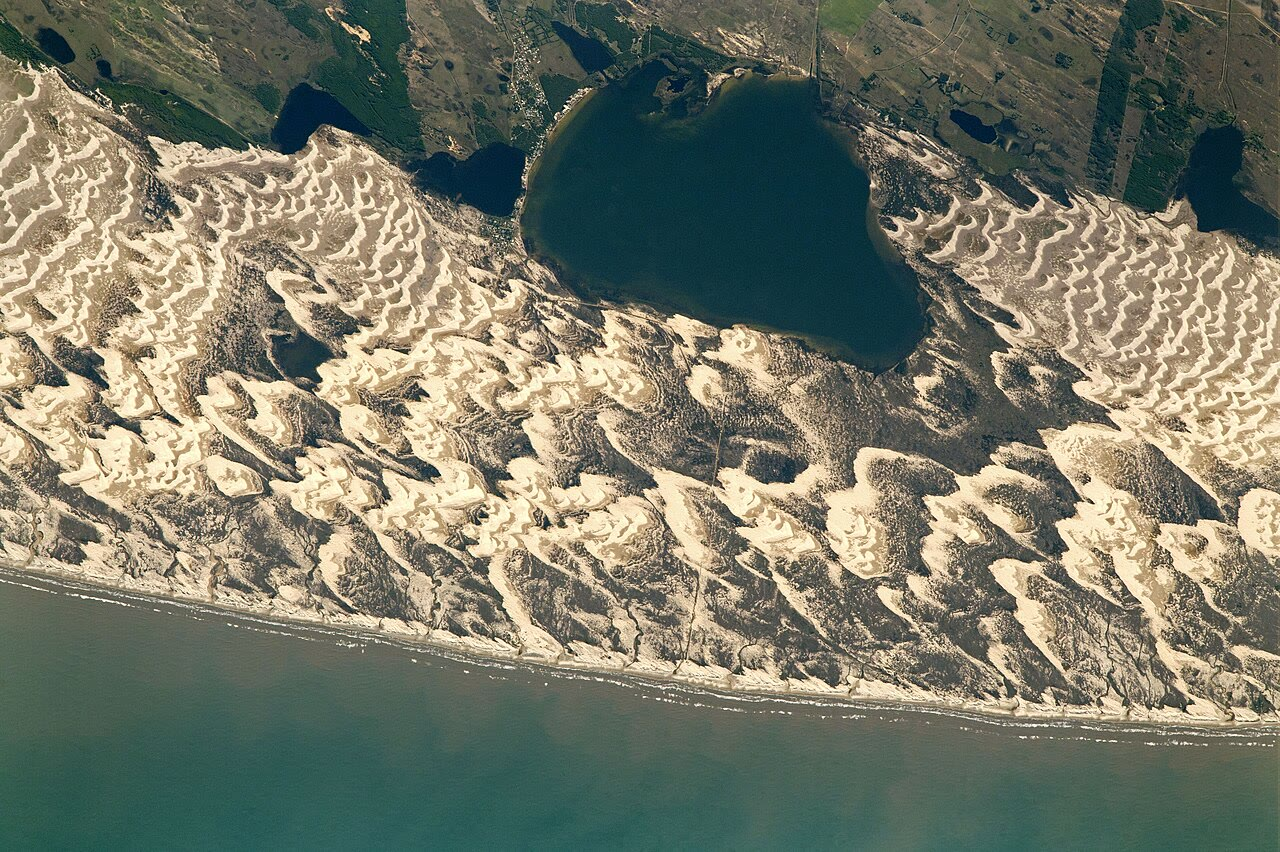
\includegraphics[width=\linewidth]{images/book1/g9-barchans.jpg}
\end{minipage}\hfill
\begin{minipage}[c]{0.46\linewidth}\raggedright
{\small \omterm{def:g9:landforms:dune}{Dunas} em crescente na costa atlântica do sul do Brasil,
fotografadas por um astronauta da Estação Espacial Internacional em 2017.
A lagoa escura, a Lagoa dos Barros, tem cerca de \qty{4.5}{km} de
comprimento. A \omterm{def:g3:stones-pebbles-sand:sand}{areia} vem da \omterm{def:g9:landforms:beach}{praia}, na parte de baixo da fotografia. NASA
(domínio público, via Wikimedia Commons).}
\end{minipage}
% ledger: commons:iss-barchans
\label{fig:g9:landforms:barchans-photo}
\end{omfigure}

Numa costa, uma linha de \omterm{def:g9:landforms:dune}{dunas} atrás da \omterm{def:g9:landforms:beach}{praia} protege a terra que fica
atrás dela das ondas de \omterm{def:g5:natural-hazards:storm}{tempestade}. As plantas que crescem nas \omterm{def:g9:landforms:dune}{dunas}
seguram a \omterm{def:g3:stones-pebbles-sand:sand}{areia} com as suas raízes: onde elas são pisoteadas ou
arrancadas, o vento leva a \omterm{def:g3:stones-pebbles-sand:sand}{areia} de novo.
% ledger: nps:aeolian

\section{As formas feitas pelo mar}

\subsection{As falésias}

\begin{definition}[Falésia]\label{def:g9:landforms:cliff}
Uma \emph{falésia}\index{falesia@falésia} é uma parede de \omterm{def:g3:stones-pebbles-sand:rock}{rocha} íngreme
ou vertical. Numa costa, uma falésia é escavada pelas ondas, que atacam o
seu pé e a fazem recuar para o interior.
\end{definition}

As ondas lançam água, \omterm{def:g3:stones-pebbles-sand:sand}{areia} e \omterm{def:g3:stones-pebbles-sand:pebble}{seixos} contra o pé da \omterm{def:g9:landforms:cliff}{falésia}. Pouco a
pouco, elas escavam uma reentrância na sua base, um \emph{entalhe}, entre
os níveis da maré baixa e da maré alta. A \omterm{def:g3:stones-pebbles-sand:rock}{rocha} de cima fica em balanço;
a \omterm{def:g4:clouds-rain-snow:precipitation}{chuva} e o gelo a enfraquecem ainda mais. Um dia, a parte em balanço
desaba. As ondas quebram os blocos caídos e os levam embora, e o ataque
recomeça numa face nova, um pouco mais para o interior. Atrás dela, a
\omterm{def:g9:landforms:cliff}{falésia} deixa uma laje plana de \omterm{def:g3:stones-pebbles-sand:rock}{rocha}, a \emph{plataforma de
abrasão}\index{plataforma de abrasao@plataforma de abrasão}, que aparece
na maré baixa.
% ledger: nt:birling-2014, sdnp:birling

As \omterm{def:g3:stones-pebbles-sand:rock}{rochas} moles recuam mais depressa. Em Birling Gap, as \omterm{def:g9:landforms:cliff}{falésias} de giz
perdem até cerca de um metro por ano; mas o recuo vem aos saltos, um
desmoronamento de cada vez, e um inverno de \omterm{def:g5:natural-hazards:storm}{tempestades} pode levar anos
de recuo de uma só vez. Em 1999, o antigo farol de Belle Tout, construído
em 1832 no alto das \omterm{def:g9:landforms:cliff}{falésias} ali perto, foi deslocado \qty{17}{m} para
trás da borda, inteiro, porque a \omterm{def:g9:landforms:cliff}{falésia} estava chegando perto demais.
% ledger: sdnp:birling, nt:birling-2014

\begin{omfigure}
\begin{tikzpicture}[font=\footnotesize, >={Stealth[length=2mm]}]
  % panel 1: the notch
  \begin{scope}
    \fill[omSea!45] (0,-0.1) rectangle (1.8,0.75);
    \fill[omSea!45] (1.8,0.35) -- (2.25,0.55) -- (1.8,0.95) -- cycle;
    \fill[black!8] (1.6,-0.1) -- (1.8,0.25) -- (1.8,0.35) -- (2.25,0.55) -- (1.8,0.95) -- (1.8,2.4) -- (3.6,2.4) -- (3.6,-0.6) -- (0,-0.6) -- (0,-0.1) -- cycle;
    \draw[black!70] (0,-0.1) -- (1.6,-0.1) -- (1.8,0.25) -- (1.8,0.35) -- (2.25,0.55) -- (1.8,0.95) -- (1.8,2.4) -- (3.6,2.4);
    \foreach \y in {0.8,1.3,1.8} \draw[black!25] (1.8,\y) -- (3.6,\y);
    \fill[green!35!black!50] (1.8,2.4) rectangle (3.6,2.5);
    \draw[->, omSea!80!black, thick] (0.4,0.6) -- (1.6,0.6);
    \node[anchor=south, align=center] at (0.9,0.8) {ondas};
    \draw[black!70] (2.15,0.55) -- (2.9,1.0) node[anchor=west, fill=white, inner sep=1pt] {entalhe};
    \node[anchor=north, align=center] at (1.8,-0.7) {1. as ondas escavam\\um entalhe};
    \node[anchor=south, font=\footnotesize] at (2.7,2.5) {giz};
  \end{scope}
  % panel 2: collapse
  \begin{scope}[xshift=4.6cm]
    \fill[omSea!45] (0,-0.1) rectangle (2.2,0.75);
    \fill[black!8] (2.0,-0.1) -- (2.2,0.25) -- (2.25,2.4) -- (3.6,2.4) -- (3.6,-0.6) -- (0,-0.6) -- (0,-0.1) -- cycle;
    \draw[black!70] (0,-0.1) -- (2.0,-0.1) -- (2.2,0.25) -- (2.25,2.4) -- (3.6,2.4);
    \draw[black!50, dashed] (1.8,0.95) -- (1.8,2.4) -- (2.25,2.4);
    \foreach \y in {0.8,1.3,1.8} \draw[black!25] (2.25,\y) -- (3.6,\y);
    \fill[green!35!black!50] (2.25,2.4) rectangle (3.6,2.5);
    \foreach \x/\y/\s in {1.25/0.05/0.28, 1.6/0.1/0.22, 1.95/0.3/0.3, 1.45/0.35/0.18}
      \fill[black!20, draw=black!60] (\x,\y) rectangle ++(\s,\s*0.8);
    \node[anchor=north, align=center] at (1.8,-0.7) {2. a parte em balanço\\desaba};
  \end{scope}
  % panel 3: retreat and platform
  \begin{scope}[xshift=9.2cm]
    \fill[omSea!45] (0,0.2) rectangle (2.8,0.75);
    \fill[black!8] (0,0.0) -- (2.6,0.2) -- (2.8,0.3) -- (2.85,2.4) -- (4.0,2.4) -- (4.0,-0.6) -- (0,-0.6) -- cycle;
    \draw[black!70] (0,0.0) -- (2.6,0.2) -- (2.8,0.3) -- (2.85,2.4) -- (4.0,2.4);
    \foreach \y in {0.8,1.3,1.8} \draw[black!25] (2.85,\y) -- (4.0,\y);
    \fill[green!35!black!50] (2.85,2.4) rectangle (4.0,2.5);
    \draw[black!50, dashed] (1.4,0.12) -- (1.4,2.4);
    \draw[black!50, dashed] (2.1,0.16) -- (2.1,2.4);
    \draw[<-, thick] (2.8,1.6) -- (1.5,1.6);
    \node[anchor=south, align=center] at (1.4,2.45) {antigas faces da falésia};
    \node[anchor=north, align=center] at (2.0,-0.7) {3. uma plataforma de abrasão,\\descoberta na maré baixa};
  \end{scope}
\end{tikzpicture}

{\small Como uma \omterm{def:g9:landforms:cliff}{falésia} marinha recua (um esboço, fora de escala). (1) As
ondas escavam um entalhe no pé da \omterm{def:g9:landforms:cliff}{falésia}. (2) A \omterm{def:g3:stones-pebbles-sand:rock}{rocha} em balanço desaba;
as ondas quebram os blocos e os levam embora. (3) O ciclo se repete: a
\omterm{def:g9:landforms:cliff}{falésia} avança para o interior e deixa uma plataforma de \omterm{def:g3:stones-pebbles-sand:rock}{rocha} plana à
sua frente.}
% ledger: nt:birling-2014, sdnp:birling
\label{fig:g9:landforms:cliff-retreat}
\end{omfigure}

\begin{safety}
A borda de uma \omterm{def:g9:landforms:cliff}{falésia} pode ceder a qualquer momento, e \omterm{def:g3:stones-pebbles-sand:rock}{rochas} caem da
parede sem aviso. As \omterm{def:g9:landforms:cliff}{falésias} são observadas de uma distância segura:
bem longe da borda, no alto, e bem longe do pé, na \omterm{def:g9:landforms:beach}{praia}; e uma \omterm{def:g9:landforms:beach}{praia} ao
pé de \omterm{def:g9:landforms:cliff}{falésias} é deixada antes de a maré subir.
\end{safety}
% ledger: nt:birling-2014, sdnp:birling

\subsection{As praias e os pontais}

A \omterm{def:g3:stones-pebbles-sand:sand}{areia} e os \omterm{def:g3:stones-pebbles-sand:pebble}{seixos} arrancados das \omterm{def:g9:landforms:cliff}{falésias}, e trazidos pelos \omterm{def:g1:landscapes-around-us:water}{rios}, não
ficam onde caem: as ondas os separam e os deslocam ao longo da costa.

\begin{definition}[Praia, deriva litorânea e pontal]\label{def:g9:landforms:beach}
Uma \emph{praia}\index{praia} é uma faixa de \omterm{def:g3:stones-pebbles-sand:sand}{areia} ou de \omterm{def:g3:stones-pebbles-sand:pebble}{seixos} acumulada
pelas ondas ao longo da margem. Quando as ondas chegam à margem de
viés, cada onda empurra os grãos praia acima nesse ângulo, e a água volta
direto descendo a encosta: os grãos fazem zigue-zague ao longo da costa.
Esse movimento da \omterm{def:g3:stones-pebbles-sand:sand}{areia} e dos \omterm{def:g3:stones-pebbles-sand:pebble}{seixos} ao longo da margem é a \emph{deriva
litorânea}\index{deriva litoranea@deriva litorânea}. Um
\emph{pontal}\index{pontal} é uma crista longa e estreita de \omterm{def:g3:stones-pebbles-sand:sand}{areia} ou de
\omterm{def:g3:stones-pebbles-sand:pebble}{seixos} construída pela deriva litorânea, presa à terra por uma ponta e
avançando \omterm{def:g2:water-on-earth:ocean}{mar} adentro onde a costa faz uma curva.
\end{definition}
% ledger: noaa:longshore

Onde a costa se curva, na entrada de uma baía ou na \omterm{def:g5:water-shapes-the-land:source-mouth}{foz} de um \omterm{def:g1:landscapes-around-us:water}{rio}, a
deriva continua no mesmo sentido e deixa a sua carga na água mais calma:
a \omterm{def:g9:landforms:beach}{praia} cresce \omterm{def:g2:water-on-earth:ocean}{mar} adentro como um \omterm{def:g9:landforms:beach}{pontal}. A sua ponta muitas vezes se
curva para dentro, dobrada por ondas que vêm de outras direções. Atrás do
\omterm{def:g9:landforms:beach}{pontal}, abrigada das ondas, a \omterm{def:g3:stones-pebbles-sand:sand}{lama} se deposita e crescem marismas.
% ledger: noaa:longshore

\begin{omfigure}
\begin{tikzpicture}[font=\footnotesize, >={Stealth[length=2mm]}]
  % sea
  \fill[omSea!40] (0,0) rectangle (11,2.3);
  % land with a bay
  \fill[green!25!black!20] (0,2.3) -- (6,2.3) .. controls (6.3,3.0) and (7.0,3.5) .. (8.0,3.5)
     .. controls (9.0,3.5) and (9.3,2.8) .. (9.5,2.3) -- (11,2.3) -- (11,4.6) -- (0,4.6) -- cycle;
  % calm water of the bay
  \fill[omSea!20] (6,2.3) .. controls (6.3,3.0) and (7.0,3.5) .. (8.0,3.5)
     .. controls (9.0,3.5) and (9.3,2.8) .. (9.5,2.3) -- cycle;
  % salt marsh
  \fill[green!50!black!35] (6.15,2.55) .. controls (6.6,3.1) and (7.3,3.2) .. (7.9,3.0)
     .. controls (7.6,2.7) and (7.0,2.6) .. (6.15,2.55) -- cycle;
  \node[anchor=west, font=\scriptsize] at (6.5,3.85) {marisma};
  \draw[black!60] (6.9,3.75) -- (7.0,2.95);
  % river
  \draw[omRiver, line width=1.2pt] (8.6,4.6) .. controls (8.5,4.0) and (8.3,3.7) .. (8.3,3.48);
  \node[anchor=west, font=\scriptsize] at (8.65,4.25) {rio};
  % beach
  \fill[yellow!40!orange!35] (0,1.85) rectangle (6,2.3);
  % spit
  \fill[yellow!40!orange!35] (5.9,1.85) .. controls (7.0,1.95) and (7.8,2.0) .. (8.35,2.1)
     .. controls (8.6,2.2) and (8.6,2.5) .. (8.4,2.65) -- (8.25,2.55)
     .. controls (8.35,2.45) and (8.3,2.35) .. (8.15,2.32)
     .. controls (7.5,2.28) and (6.8,2.3) .. (6.0,2.3) -- cycle;
  \draw[black!60] (0,2.3) -- (6,2.3) .. controls (6.3,3.0) and (7.0,3.5) .. (8.0,3.5)
     .. controls (9.0,3.5) and (9.3,2.8) .. (9.5,2.3) -- (11,2.3);
  % waves arriving at an angle
  \foreach \x in {0.9,2.0,3.1,4.2} \draw[omSea!70!black, line width=0.5pt] (\x,1.15) -- ++(-35:1.1);
  \draw[->, omSea!70!black, thick] (0.6,0.3) -- ++(55:1.2) node[pos=0.15, left, black] {ondas};
  % zigzag of a pebble
  \draw[->, black, thick] (1.0,1.9) -- (1.35,2.2) -- (1.35,1.9) -- (1.7,2.2) -- (1.7,1.9)
     -- (2.05,2.2) -- (2.05,1.9) -- (2.4,2.2) -- (2.4,1.9);
  \node[anchor=south, align=center, font=\scriptsize] at (1.7,2.45) {praia acima de viés,\\de volta direto\\para baixo};
  % drift arrow
  \draw[->, line width=1.6pt, omWarm] (3.0,1.55) -- (5.6,1.55) node[midway, below, black] {deriva litorânea};
  % spit label
  \draw[black!70] (7.4,2.05) -- (7.6,1.2) node[anchor=north, align=center, black] {o pontal cresce\\através da baía};
  \draw[->, thick, omWarm] (8.6,1.95) -- ++(0.6,0);
  % compass
  \draw[->] (10.4,0.3) -- ++(0,0.6) node[above] {N};
\end{tikzpicture}

{\small A \omterm{def:g9:landforms:beach}{deriva litorânea} e um \omterm{def:g9:landforms:beach}{pontal}, vistos de cima (um esboço). As
ondas chegam do sudoeste; cada uma empurra a \omterm{def:g3:stones-pebbles-sand:sand}{areia} e os \omterm{def:g3:stones-pebbles-sand:pebble}{seixos} \omterm{def:g9:landforms:beach}{praia} acima
de viés, e a água volta direto para baixo: os grãos fazem zigue-zague
para leste. Onde a costa se curva para dentro de uma baía, a deriva
continua e constrói um \omterm{def:g9:landforms:beach}{pontal}, atrás do qual cresce uma marisma. O \omterm{def:g1:landscapes-around-us:water}{rio}
mantém um canal aberto na ponta do \omterm{def:g9:landforms:beach}{pontal}.}
% ledger: noaa:longshore
\label{fig:g9:landforms:spit}
\end{omfigure}

\begin{omfigure}
\begin{minipage}[c]{0.5\linewidth}\centering
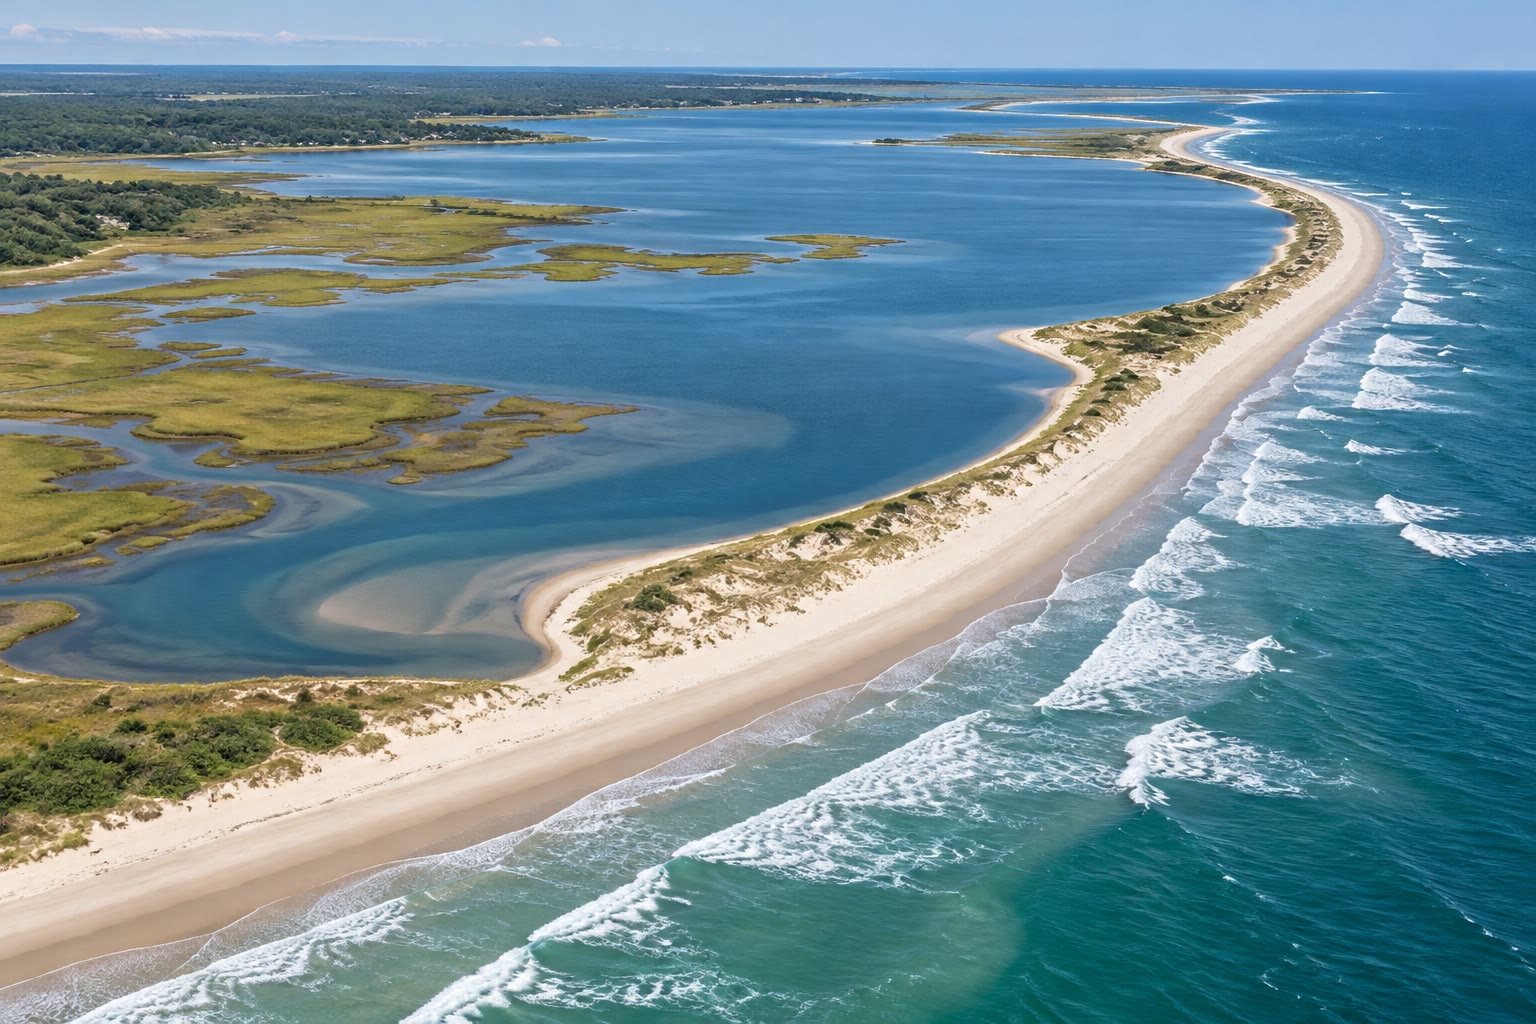
\includegraphics[width=\linewidth]{images/book1/ai/g9-spit-aerial.jpg}
\end{minipage}\hfill
\begin{minipage}[c]{0.46\linewidth}\raggedright
{\small Um \omterm{def:g9:landforms:beach}{pontal} arenoso atravessando a entrada de uma baía, visto de um
avião voando baixo (uma ilustração, não um lugar real). As ondas
arrebentam na sua \omterm{def:g9:landforms:beach}{praia} voltada para o \omterm{def:g2:water-on-earth:ocean}{mar}; atrás dele ficam águas calmas
e marismas.}
\end{minipage}
\label{fig:g9:landforms:spit-ai}
\end{omfigure}

\section{As formas feitas pela dissolução: o carste}

A água da \omterm{def:g4:clouds-rain-snow:precipitation}{chuva} não é água pura. Ao cair pelo ar e depois se infiltrar
pelo solo, ela absorve gás carbônico, que a deixa levemente ácida. Esse
ácido fraco faz devagar o que a gota de ácido diluído faz depressa com um
pedaço de calcário: ele dissolve a \omterm{def:g3:stones-pebbles-sand:rock}{rocha}. O calcário é cheio de fendas, ao
longo das suas camadas e através delas. A água desce por elas e as alarga,
milímetro por milímetro, ao longo de milhares de anos.
% ledger: usgs:sinkholes, nps:karst

\begin{definition}[Carste, caverna e dolina]\label{def:g9:landforms:karst}
Um \emph{carste}\index{carste} é uma \omterm{def:g1:landscapes-around-us:landscape}{paisagem} modelada pela água que
dissolve uma \omterm{def:g3:stones-pebbles-sand:rock}{rocha} solúvel, na maioria das vezes o calcário. Ali, os \omterm{def:g1:landscapes-around-us:water}{rios}
costumam sumir embaixo da terra e voltar à superfície como \omterm{def:g5:water-shapes-the-land:source-mouth}{nascentes}.
Uma \emph{caverna}\index{caverna} é um espaço subterrâneo natural grande
o bastante para uma pessoa entrar, dissolvido ao longo das fendas da
\omterm{def:g3:stones-pebbles-sand:rock}{rocha}. Uma \emph{dolina}\index{dolina} é uma depressão ou um buraco na
superfície do terreno, formado onde a \omterm{def:g3:stones-pebbles-sand:rock}{rocha} de baixo se dissolve ou onde
o teto de uma caverna desaba.
\end{definition}
% ledger: nps:karst, usgs:sinkholes

\begin{omfigure}
\begin{tikzpicture}[x=0.9cm, y=0.9cm, font=\footnotesize, >={Stealth[length=2mm]}]
  \pic (B) at (0,0) {blockdiagram={10}{4}{4}};
  % top face: grassland
  \fill[green!25!black!18] (B-ftl) -- (B-ftr) -- (B-btr) -- (B-btl) -- cycle;
  % right face
  \fill[omLithLime!70] (B-fbr) -- (B-bbr) -- (B-btr) -- (B-ftr) -- cycle;
  % front face: limestone layers
  \fill[omLithLime] (B-fbl) rectangle (B-ftr);
  \foreach \y in {0.8,1.6,2.4,3.2} \draw[black!35] (0,\y) -- (10,\y);
  \foreach \x/\y in {1.2/0.8, 3.1/1.6, 4.6/0, 6.8/2.4, 8.3/0.8, 2.2/2.4, 9.1/2.4, 5.6/3.2}
    \draw[black!35] (\x,\y) -- ++(0,0.8);
  % soil
  \fill[brown!45] (0,3.8) rectangle (10,4);
  % sinkhole on the top face and in the front face
  \fill[green!25!black!35] (3.0,4.45) ellipse (0.7 and 0.22);
  \fill[white] (2.3,4) -- (3.7,4) -- (3.25,3.45) -- (2.75,3.45) -- cycle;
  \fill[green!25!black!30] (2.3,4) -- (3.7,4) -- (3.25,3.45) -- (2.75,3.45) -- cycle;
  \draw[black!60] (2.3,4) -- (2.75,3.45) -- (3.25,3.45) -- (3.7,4);
  % shaft from sinkhole to cave
  \fill[white] (2.85,3.45) -- (3.15,3.45) -- (3.35,2.0) -- (3.05,2.0) -- cycle;
  \draw[black!60] (2.85,3.45) -- (3.05,2.0) (3.15,3.45) -- (3.35,2.0);
  % cave
  \fill[white] (2.6,2.1) .. controls (3.5,2.35) and (5.5,2.3) .. (6.6,1.9)
     .. controls (7.4,1.6) and (7.6,1.2) .. (7.2,1.0)
     .. controls (6.0,0.85) and (4.0,1.0) .. (3.0,1.2)
     .. controls (2.3,1.35) and (2.1,1.9) .. (2.6,2.1) -- cycle;
  \draw[black!70] (2.6,2.1) .. controls (3.5,2.35) and (5.5,2.3) .. (6.6,1.9)
     .. controls (7.4,1.6) and (7.6,1.2) .. (7.2,1.0)
     .. controls (6.0,0.85) and (4.0,1.0) .. (3.0,1.2)
     .. controls (2.3,1.35) and (2.1,1.9) .. (2.6,2.1);
  % underground stream at the cave floor
  \fill[omRiver!60] (3.0,1.2) .. controls (4.0,1.0) and (6.0,0.85) .. (7.2,1.0) -- (7.1,1.12)
     .. controls (6.0,1.0) and (4.0,1.12) .. (3.1,1.3) -- cycle;
  % stalactites and stalagmites
  \foreach \x/\l in {4.2/0.35, 4.5/0.22, 4.9/0.4, 5.3/0.25, 5.8/0.3}
    \fill[black!45] (\x-0.07,2.22) -- (\x+0.06,2.22) -- (\x,2.22-\l) -- cycle;
  \foreach \x/\l in {4.9/0.3, 5.8/0.25}
    \fill[black!45] (\x-0.12,0.95) -- (\x+0.12,0.95) -- (\x,0.95+\l) -- cycle;
  % disappearing stream on the top face
  \draw[omRiver, line width=1.2pt] (7.4,4.85) .. controls (6.9,4.5) and (6.4,4.4) .. (6.0,4.25);
  \fill[black!70] (6.0,4.25) circle (0.07);
  \draw[omRiver, dashed, thick] (6.0,4.0) -- (6.4,2.1);
  % spring on the right face
  \draw[omRiver, line width=1.2pt, ->] (10.2,1.2) .. controls (10.8,1.1) and (11.2,0.7) .. (11.6,0.5);
  % rain with carbon dioxide
  \foreach \x in {0.6,1.2,1.8} \draw[->, omRiver] (\x,5.6) -- ++(-0.15,-0.7);
  \draw[->, omRiver, dashed] (1.0,3.9) -- (1.2,1.7);
  % outline
  \draw[black!70] (B-fbl) rectangle (B-ftr);
  \draw[black!70] (B-ftl) -- (B-btl) -- (B-btr) -- (B-ftr) (B-btr) -- (B-bbr) -- (B-fbr);
  % labels
  \node[anchor=south, align=center] at (1.2,5.6) {a chuva absorve\\gás carbônico:\\levemente ácida};
  \node[anchor=east, align=right] at (-0.1,1.6) {a água alarga\\as fendas};
  \draw[black!70] (-0.05,1.6) -- (1.1,2.0);
  \node[anchor=south] at (3.0,5.2) {dolina};
  \draw[black!70] (3.0,5.2) -- (3.0,4.55);
  \node[anchor=south, align=center] at (7.6,5.3) {um riacho some\\embaixo da terra};
  \draw[black!70] (7.0,5.3) -- (6.1,4.35);
  \node[anchor=north, align=center] at (5.0,-0.1) {uma caverna: as estalactites pendem do teto,\\as estalagmites sobem do chão};
  \draw[black!70] (5.0,-0.1) -- (5.0,1.4);
  \node[anchor=west, align=left] at (11.6,0.6) {nascente};
  \node[anchor=west] at (11.9,3.4) {calcário};
\end{tikzpicture}

{\small Uma \omterm{def:g1:landscapes-around-us:landscape}{paisagem} cárstica (um esboço, fora de escala). A água levemente
ácida se infiltra pelas fendas do calcário e as alarga; riachos
subterrâneos escavam \omterm{def:g9:landforms:karst}{cavernas}; o teto de uma \omterm{def:g9:landforms:karst}{caverna} cede e abre uma
\omterm{def:g9:landforms:karst}{dolina}; um riacho some num buraco e volta à superfície como \omterm{def:g5:water-shapes-the-land:source-mouth}{nascente} mais
abaixo.}
% ledger: nps:karst, usgs:sinkholes, nps:speleothems
\label{fig:g9:landforms:karst}
\end{omfigure}

Numa \omterm{def:g9:landforms:karst}{caverna}, a dissolução pode andar para trás. Uma gota de água que
pinga do teto leva calcário dissolvido. Quando encontra o ar da \omterm{def:g9:landforms:karst}{caverna},
ela libera parte do seu gás carbônico, e uma fina película de calcita sai
da água em volta da gota. Gota após gota, um tubo oco cresce a partir do
teto e depois engrossa até virar uma \emph{estalactite}\index{estalactite},
pendurada como um pingente de gelo. Onde as gotas caem, o resto da calcita
constrói uma \emph{estalagmite}\index{estalagmite} a partir do chão.
Quando as duas se encontram, formam uma coluna.
% ledger: nps:speleothems

\begin{omfigure}
\begin{minipage}[c]{0.5\linewidth}\centering
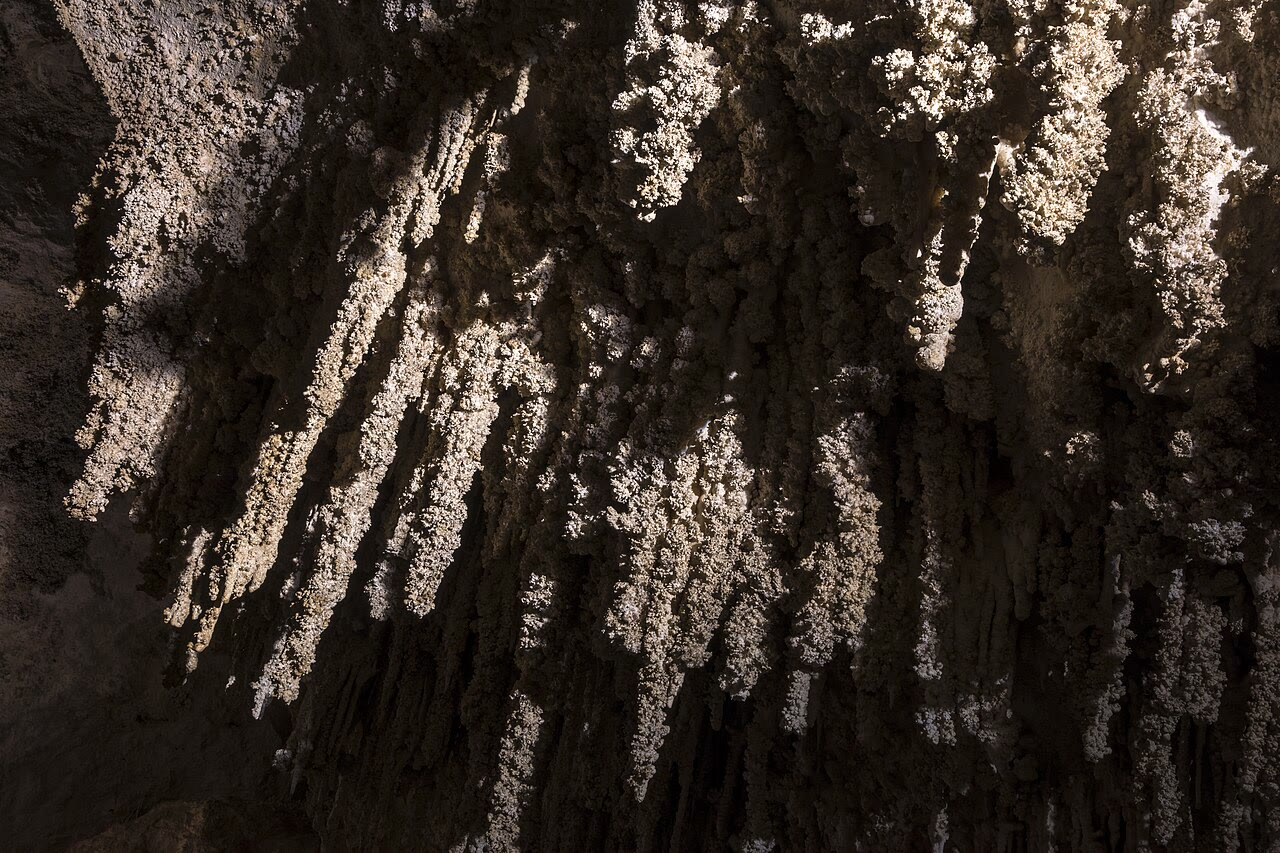
\includegraphics[width=\linewidth]{images/book1/g9-stalactites.jpg}
\end{minipage}\hfill
\begin{minipage}[c]{0.46\linewidth}\raggedright
{\small Estalactites penduradas embaixo de um grande bloco de \omterm{def:g3:stones-pebbles-sand:rock}{rocha} na
Carlsbad Cavern, no Novo México, uma \omterm{def:g9:landforms:karst}{caverna} dissolvida no calcário. Cada
uma cresceu gota a gota a partir da água que se infiltra pela \omterm{def:g3:stones-pebbles-sand:rock}{rocha} de
cima. National Park Service, 2018 (domínio público, via Wikimedia
Commons).}
\end{minipage}
% ledger: commons:carlsbad-stalactites, nps:speleothems
\label{fig:g9:landforms:stalactites}
\end{omfigure}

As regiões cársticas guardam muita água no subsolo, mas ela corre depressa
pelas fendas abertas e quase não é filtrada: tudo o que é derramado no
chão pode chegar depressa a uma \omterm{def:g5:water-shapes-the-land:source-mouth}{nascente}. E, onde a \omterm{def:g3:stones-pebbles-sand:rock}{rocha} de baixo foi
dissolvida, o terreno pode afundar ou desabar: onde há gente morando, uma
\omterm{def:g9:landforms:karst}{dolina} que se abre de repente pode engolir estradas e casas.
% ledger: nps:karst, usgs:sinkholes

\section{Ler uma paisagem}

Cada \omterm{def:g1:landscapes-around-us:landform}{forma de relevo} é uma pista. A sua forma diz que agente a fez; o
agente diz que processo atuou, \omterm{def:g5:water-shapes-the-land:erosion}{erosão} ou \omterm{def:g5:water-shapes-the-land:deposition}{deposição}; e o processo muitas
vezes diz algo sobre a \omterm{def:g3:stones-pebbles-sand:rock}{rocha} ou sobre o material solto que fica embaixo.

\begin{method}[Ler uma forma de relevo]
\begin{enumerate}
  \item \textbf{Forma.} Descreva a \omterm{def:g1:landscapes-around-us:landform}{forma de relevo}: uma crista, uma
        depressão, uma parede íngreme, uma laje plana; o seu tamanho; para
        onde ela aponta.
  \item \textbf{Agente e processo.} Decida que agente a fez (um \omterm{def:g1:landscapes-around-us:water}{rio}, o
        gelo, o vento, o \omterm{def:g2:water-on-earth:ocean}{mar}, a água que dissolve) e se ela foi escavada
        (\omterm{def:g5:water-shapes-the-land:erosion}{erosão}) ou construída (\omterm{def:g5:water-shapes-the-land:deposition}{deposição}).
  \item \textbf{Material.} Diga de que ela é feita, ou o que a \omterm{def:g3:stones-pebbles-sand:rock}{rocha} de
        baixo provavelmente é: \omterm{def:g3:stones-pebbles-sand:sand}{areia} solta, \omterm{def:g3:stones-pebbles-sand:pebble}{seixos}, calcário, \omterm{def:g3:stones-pebbles-sand:rock}{rocha} dura ou
        mole.
\end{enumerate}
\end{method}

\begin{center}
{\small
\begin{tabular}{|>{\raggedright\arraybackslash}p{4.6cm}|>{\raggedright\arraybackslash}p{2.6cm}|>{\raggedright\arraybackslash}p{2.2cm}|>{\raggedright\arraybackslash}p{2.6cm}|}
\hline
forma & agente & processo & material \\
\hline
morros de \omterm{def:g3:stones-pebbles-sand:sand}{areia} em crescente & vento & \omterm{def:g5:water-shapes-the-land:deposition}{deposição} & \omterm{def:g3:stones-pebbles-sand:sand}{areia} solta \\
uma parede de \omterm{def:g3:stones-pebbles-sand:rock}{rocha} vertical acima de uma laje de \omterm{def:g3:stones-pebbles-sand:rock}{rocha} plana & \omterm{def:g2:water-on-earth:ocean}{mar} & \omterm{def:g5:water-shapes-the-land:erosion}{erosão} & \omterm{def:g3:stones-pebbles-sand:rock}{rocha} (a \omterm{def:g3:stones-pebbles-sand:rock}{rocha} mole recua depressa) \\
uma crista estreita de \omterm{def:g3:stones-pebbles-sand:sand}{areia} atravessando uma baía & \omterm{def:g2:water-on-earth:ocean}{mar} (\omterm{def:g9:landforms:beach}{deriva litorânea}) & \omterm{def:g5:water-shapes-the-land:deposition}{deposição} & \omterm{def:g3:stones-pebbles-sand:sand}{areia} ou \omterm{def:g3:stones-pebbles-sand:pebble}{seixos} \\
depressões nos campos, riachos que somem & água que dissolve & dissolução & calcário \\
um \omterm{def:g8:ice-on-earth:glacial-landforms}{vale em U} & gelo & \omterm{def:g5:water-shapes-the-land:erosion}{erosão} & qualquer \omterm{def:g3:stones-pebbles-sand:rock}{rocha} \\
um leque de \omterm{def:g3:stones-pebbles-sand:sand}{lama} na \omterm{def:g5:water-shapes-the-land:source-mouth}{foz} de um \omterm{def:g1:landscapes-around-us:water}{rio} & \omterm{def:g1:landscapes-around-us:water}{rio} & \omterm{def:g5:water-shapes-the-land:deposition}{deposição} & \omterm{def:g3:stones-pebbles-sand:sand}{lama} e \omterm{def:g3:stones-pebbles-sand:sand}{areia} \\
\hline
\end{tabular}}
\end{center}

\begin{example}[Um passeio num planalto]
Num planalto alto coberto de capim, não há nenhum riacho, embora chova
muitas vezes. Os campos são salpicados de depressões redondas de alguns
metros de diâmetro, e, no \omterm{def:g1:landscapes-around-us:landform}{vale} lá embaixo, uma \omterm{def:g5:water-shapes-the-land:source-mouth}{nascente} forte jorra do pé
de uma parede de \omterm{def:g3:stones-pebbles-sand:rock}{rocha}. \emph{Forma}: depressões, nenhum riacho na
superfície, uma \omterm{def:g5:water-shapes-the-land:source-mouth}{nascente} mais abaixo. \emph{Agente e processo}: água que
dissolve a \omterm{def:g3:stones-pebbles-sand:rock}{rocha} e corre embaixo da terra. \emph{Material}: o planalto é
muito provavelmente de calcário, e as depressões são \omterm{def:g9:landforms:karst}{dolinas}. Uma gota de
ácido diluído num pedaço solto da \omterm{def:g3:stones-pebbles-sand:rock}{rocha}, posta pela professora,
efervesceria.
\end{example}
% ledger: nps:karst, usgs:sinkholes

\section{Exercícios}

\begin{exercise}[$\star$]\label{exo:g9:landforms:1}
Que agente fez cada \omterm{def:g1:landscapes-around-us:landform}{forma de relevo}: o vento, o \omterm{def:g2:water-on-earth:ocean}{mar}, um \omterm{def:g1:landscapes-around-us:water}{rio}, o gelo ou a
água que dissolve a \omterm{def:g3:stones-pebbles-sand:rock}{rocha}? (a) Um morro de \omterm{def:g3:stones-pebbles-sand:sand}{areia} em crescente num
\omterm{def:g5:weather-and-climate:desert}{deserto}. (b) Uma \omterm{def:g9:landforms:karst}{caverna} cheia de estalactites. (c) Uma longa crista de
\omterm{def:g3:stones-pebbles-sand:pebble}{seixos} atravessando a entrada de uma baía. (d) Um \omterm{def:g8:ice-on-earth:glacial-landforms}{vale em U} com uma
\omterm{def:g8:ice-on-earth:glacial-landforms}{morena} na sua ponta. (e) Uma parede vertical de giz com uma laje de \omterm{def:g3:stones-pebbles-sand:rock}{rocha}
plana ao pé. (f) Um \omterm{def:g5:water-shapes-the-land:delta}{delta}.
\end{exercise}

\begin{exercise}[$\star$]\label{exo:g9:landforms:2}
Dê a palavra de cada descrição. (a) A subida lenta das \omterm{def:g3:stones-pebbles-sand:rock}{rochas} e do
terreno de uma região. (b) O lado íngreme de uma \omterm{def:g9:landforms:dune}{duna}, oposto ao vento.
(c) Um buraco no chão formado onde a \omterm{def:g3:stones-pebbles-sand:rock}{rocha} de baixo se dissolveu ou onde
o teto de uma \omterm{def:g9:landforms:karst}{caverna} desabou. (d) O movimento da \omterm{def:g3:stones-pebbles-sand:sand}{areia} e dos \omterm{def:g3:stones-pebbles-sand:pebble}{seixos} ao
longo da margem. (e) Uma \omterm{def:g1:landscapes-around-us:landscape}{paisagem} modelada pela água que dissolve o
calcário.
\end{exercise}

\begin{exercise}[$\star$]\label{exo:g9:landforms:3}
Verdadeiro ou falso? Corrija as frases falsas. (a) Os chifres de uma \omterm{def:g9:landforms:dune}{duna}
em crescente apontam para o lado de onde vem o vento. (b) A encosta de
uma \omterm{def:g9:landforms:dune}{duna} voltada para o vento é suave. (c) Uma \omterm{def:g9:landforms:dune}{duna} se move porque o
vento a levanta toda de uma vez. (d) As \omterm{def:g9:landforms:dune}{dunas} se formam com mais
facilidade onde crescem poucas plantas.
\end{exercise}

\begin{exercise}[$\star$]\label{exo:g9:landforms:4}
Ponha em ordem estas etapas do recuo de uma \omterm{def:g9:landforms:cliff}{falésia} marinha. (a) As ondas
quebram os blocos caídos e os levam embora. (b) As ondas escavam um
entalhe no pé da \omterm{def:g9:landforms:cliff}{falésia}. (c) A parede da \omterm{def:g9:landforms:cliff}{falésia} fica agora mais para o
interior, e a plataforma plana à sua frente fica um pouco mais larga. (d)
A \omterm{def:g3:stones-pebbles-sand:rock}{rocha} acima do entalhe fica em balanço. (e) A parte em balanço desaba.
\end{exercise}

\begin{exercise}[$\star\star$]\label{exo:g9:landforms:5}
% ledger: nps:whsa-migration (6 and 3 m a year)
Vistas de um avião, as \omterm{def:g9:landforms:dune}{dunas} em crescente de um \omterm{def:g5:weather-and-climate:desert}{deserto} têm todas os
chifres apontando para leste. (a) De que direção sopra o vento? (b) De
que lado de cada \omterm{def:g9:landforms:dune}{duna} fica a \omterm{def:g9:landforms:dune}{face de avalanche}? (c) Uma estrada passa
\qty{60}{m} a leste de uma das \omterm{def:g9:landforms:dune}{dunas}. A \omterm{def:g9:landforms:dune}{duna} avança \qty{6}{m} por ano. Em
quantos anos o seu pé vai chegar à estrada? (d) Uma \omterm{def:g9:landforms:dune}{duna} maior avança só
\qty{3}{m} por ano. Por que as \omterm{def:g9:landforms:dune}{dunas} maiores se movem mais devagar?
\end{exercise}

\begin{exercise}[$\star\star$]\label{exo:g9:landforms:6}
% ledger: sdnp:birling, nt:birling-2014
As \omterm{def:g9:landforms:cliff}{falésias} de giz de uma costa recuam até cerca de \qty{1}{m} por ano.
No inverno de 2014, elas perderam tanto quanto costumam perder em sete
anos, em apenas dois meses. (a) A \qty{1}{m} por ano, quanto se perde em
sete anos? (b) Dois meses são que fração de um ano? (c) Quantas vezes
mais depressa do que o normal as \omterm{def:g9:landforms:cliff}{falésias} recuaram durante esses dois
meses? (d) Explique, usando o entalhe e a parte em balanço, por que uma
\omterm{def:g9:landforms:cliff}{falésia} recua aos saltos e não de maneira contínua.
\end{exercise}

\begin{exercise}[$\star\star$]\label{exo:g9:landforms:7}
Uma costa retilínea vai de oeste a leste, com o \omterm{def:g2:water-on-earth:ocean}{mar} ao sul. As ondas vêm
do sudoeste. (a) Em que sentido a \omterm{def:g9:landforms:beach}{deriva litorânea} leva a \omterm{def:g3:stones-pebbles-sand:sand}{areia}? (b)
Desenhe o caminho em zigue-zague de um \omterm{def:g3:stones-pebbles-sand:pebble}{seixo} durante três ondas,
indicando o trajeto \omterm{def:g9:landforms:beach}{praia} acima e o trajeto de volta. (c) Na sua ponta
leste, a costa vira para o norte, para dentro de uma baía. Que \omterm{def:g1:landscapes-around-us:landform}{forma de
relevo} provavelmente vai crescer ali? (d) Por que a \omterm{def:g3:stones-pebbles-sand:sand}{lama} se deposita atrás
dela?
\end{exercise}

\begin{exercise}[$\star\star$]\label{exo:g9:landforms:8}
(a) O que deixa a água da \omterm{def:g4:clouds-rain-snow:precipitation}{chuva} levemente ácida? (b) Por que há \omterm{def:g9:landforms:karst}{cavernas}
no calcário, mas quase nenhuma no granito? (c) Por que as \omterm{def:g9:landforms:karst}{cavernas} seguem
as fendas e as camadas da \omterm{def:g3:stones-pebbles-sand:rock}{rocha}? (d) Dê duas maneiras como uma \omterm{def:g9:landforms:karst}{dolina}
pode se formar.
\end{exercise}

\begin{exercise}[$\star\star$]\label{exo:g9:landforms:9}
(a) Explique por que a calcita sai de uma gota de água pendurada no teto
de uma \omterm{def:g9:landforms:karst}{caverna}. (b) Por que as estalagmites não têm tubo oco por dentro,
ao contrário das estalactites jovens? (c) Suponha que uma estalactite
tenha crescido \qty{0.1}{mm} por ano (um ritmo inventado: os ritmos reais
variam muito). Quantos anos ela levou para crescer \qty{30}{cm}? Escreva
a resposta em notação científica.
\end{exercise}

\begin{exercise}[$\star\star$]\label{exo:g9:landforms:10}
% ledger: usgs:himalaya, sdnp:birling
O planalto do Tibete subiu cerca de \qty{4600}{m} em cerca de 10~milhões
de anos. (a) Calcule o \omterm{def:g9:landforms:uplift}{soerguimento} médio em metros por ano, em notação
científica, e depois em milímetros por ano. (b) Suponha que a \omterm{def:g5:water-shapes-the-land:erosion}{erosão}
retire \qty{0.2}{mm} por ano do planalto (um número inventado). Quanto o
planalto sobe a cada ano? (c) Uma \omterm{def:g9:landforms:cliff}{falésia} de giz recua cerca de
\qty{1}{m} por ano. Quantas vezes isso é mais rápido do que o
\omterm{def:g9:landforms:uplift}{soerguimento} de (a)? (d) Por que um \omterm{def:g9:landforms:uplift}{soerguimento} lento ainda pode
construir um planalto alto?
\end{exercise}

\begin{exercise}[$\star\star\star$]\label{exo:g9:landforms:11}
Leia cada \omterm{def:g1:landscapes-around-us:landscape}{paisagem} com o método do capítulo (forma, agente e processo,
material). (a) Numa região seca, longas fileiras de morros de \omterm{def:g3:stones-pebbles-sand:sand}{areia}, cada
um com a forma de um crescente, com um lado íngreme voltado para o
sudeste. (b) Ao pé de uma \omterm{def:g9:landforms:cliff}{falésia} branca, uma laje de \omterm{def:g3:stones-pebbles-sand:rock}{rocha} plana coberta
de algas aparece na maré baixa. (c) Num planalto largo de \omterm{def:g3:stones-pebbles-sand:rock}{rocha} clara, um
riacho atravessa um campo e some num buraco; uma \omterm{def:g5:water-shapes-the-land:source-mouth}{nascente} jorra da
encosta de um \omterm{def:g1:landscapes-around-us:landform}{vale} a \qty{2}{km} dali.
\end{exercise}

\begin{exercise}[$\star\star\star$]\label{exo:g9:landforms:12}
% ledger: nps:whsa-migration, nmt:barchan, nps:aeolian
Num campo de \omterm{def:g9:landforms:dune}{dunas}, as pequenas \omterm{def:g9:landforms:dune}{dunas} da borda a barlavento avançam até
\qty{6}{m} por ano; um pouco mais adiante, as \omterm{def:g9:landforms:dune}{dunas}, com 6 a \qty{10}{m}
de altura, avançam cerca de \qty{3}{m} por ano. Uma trilha atravessa o
campo \qty{45}{m} a sotavento de uma \omterm{def:g9:landforms:dune}{duna} de cada tipo. (a) Depois de
quantos anos cada \omterm{def:g9:landforms:dune}{duna} chega à trilha? (b) \omterm{def:g9:landforms:dune}{Dunas} empurradas por ventos
fortes podem percorrer mais de \qty{100}{m} em um ano. Quanto tempo uma
\omterm{def:g9:landforms:dune}{duna} assim levaria para cobrir a mesma distância? (c) Cite uma maneira de
frear as \omterm{def:g9:landforms:dune}{dunas}, e explique como ela funciona.
\end{exercise}

\section{Problema: A falésia e a estrada costeira}

\begin{problem}[{Problema de fim de semana --- uma estrada costeira passa
atrás de uma falésia de giz que recua; a resposta final é o ano em que a
borda da falésia chegaria à estrada no ritmo medido}]
\label{pb:g9:landforms:1}
% ledger: (invented region: exercise data, figdata/grade-9/cliff_retreat.py; the rate is kept within sdnp:birling, the storm winter recalls nt:birling-2014)
Uma estrada costeira passa pelo alto de \omterm{def:g9:landforms:cliff}{falésias} de giz. A cada poucos
anos, uma equipe de levantamento mede a distância da estrada até a borda
da \omterm{def:g9:landforms:cliff}{falésia} ao longo da mesma linha, a partir de marcos fixos colocados bem
recuados da borda, nunca na própria borda. Aqui estão as suas medidas.

\begin{center}
{\small
\begin{tabular}{|l|c|c|c|c|c|c|c|}
\hline
ano & 2004 & 2008 & 2012 & 2014 & 2016 & 2020 & 2024 \\
\hline
distância da estrada à borda (m) & 46.0 & 43.1 & 41.0 & 36.2 & 35.5 & 33.0 & 30.4 \\
\hline
\end{tabular}}
\end{center}

\noindent\textbf{Parte I --- As medidas.}\par\nopagebreak
\begin{enumerate}[beginpenalty=10000]
  \item Quantos metros a borda da \omterm{def:g9:landforms:cliff}{falésia} se aproximou da estrada entre
        2004 e 2024?
  \item Calcule o ritmo médio de recuo ao longo desses 20 anos, em metros
        por ano.
  \item Entre quais dois levantamentos a borda recuou mais depressa?
        Calcule o ritmo nesse intervalo.
  \item Quantas vezes ele é mais rápido que a média? Sugira o que
        aconteceu durante esse intervalo.
\end{enumerate}

\begin{omfigure}
\begin{tikzpicture}
\begin{axis}[omrecord, width=11cm, height=4.6cm, xmin=2000, xmax=2070,
  ymin=0, ymax=50, xtick={2000,2010,...,2070}, ytick={0,10,...,50},
  x tick label style={/pgf/number format/1000 sep={}},
  xlabel={ano}, ylabel={distância até a estrada (m)}]
  \addplot[omWarm, thick, mark=*, mark size=1.8pt] table[x=year, y=dist_m] {figdata/out/grade-9-cliff_retreat.dat};
\end{axis}
\end{tikzpicture}

{\small O levantamento: distância da estrada costeira até a borda da
\omterm{def:g9:landforms:cliff}{falésia} (dados do exercício).}
\label{fig:g9:landforms:survey}
\end{omfigure}

\noindent\textbf{Parte II --- O ritmo.}\par\nopagebreak
\begin{enumerate}[resume, beginpenalty=10000]
  \item Escreva o ritmo médio em centímetros por ano e depois em metros
        por século.
  \item Numa costa de giz real, as \omterm{def:g9:landforms:cliff}{falésias} recuam até cerca de um metro
        por ano. O recuo desta \omterm{def:g9:landforms:cliff}{falésia} tem o mesmo tamanho?
  \item Um farol numa costa assim foi um dia deslocado \qty{17}{m} para
        trás da borda. No ritmo médio desta \omterm{def:g9:landforms:cliff}{falésia}, quantos anos de recuo
        \qty{17}{m} representam?
  \item Por que o ritmo medido ao longo de 20 anos é um guia melhor para o
        futuro do que o ritmo medido ao longo de dois anos?
\end{enumerate}

\noindent\textbf{Parte III --- A estrada.}\par\nopagebreak
\begin{enumerate}[resume, beginpenalty=10000]
  \item A estrada deve ser deslocada antes que a borda chegue a menos de
        \qty{10}{m} dela. Em que ano, no ritmo médio, isso vai acontecer?
  \item Se invernos com mais \omterm{def:g5:natural-hazards:storm}{tempestades} dobrassem o ritmo, em que ano a
        borda chegaria à estrada?
  \item Por que a equipe de levantamento faz as suas medidas a partir de
        marcos colocados bem recuados da borda?
  \item No ritmo médio, em que ano a borda da \omterm{def:g9:landforms:cliff}{falésia} chegaria à estrada?
\end{enumerate}
\end{problem}
